\chapter{Методы исследования}\label{ch:ch2}

\section{Алгоритмы и методы}\label{sec:ch1/sec3}

Предложенная игровая динамика предполагает наличие двух игроков, осуществляющих свой выбор на каждом ходу исходя из некоторой стратегии.
Одним из вариантов стратегии игроков может выступать случайный равновероятный выбор одной из кнопок на каждом ходу.
Применение такой стратегии обоими игроками сводит игру к чистому случайному блужданию на ограниченной решетке -- обозначим такой случай как BvB (Bot vs Bot).
Второй вариант состоит в игре человека, применяющего произвольную стратегию, против стратегии равновероятного выбора независимо от состояния -- обозначим как PvE (Player vs Environment).
В этом случае различаются две стороны игры в зависимости от цели: как можно скорее достичь границу (игра за границу) и
как можно дольше оставаться внутри поля (игра за центр). Последний рассмотренный вариант состоит в игре двух игроков, 
выбирающих произвольные стратегии (PvP -- Player vs Player).

\subsection{Марковские цепи}\label{subsec:ch1/sec3/sub1}

Основным математическим подходом к анализу игровой динамики была выбрана теория цепей Маркова \cite{markov_chain}.
Цепь Маркова характеризует дискретный (во времени) случайный процесс, в котором вероятность наступления каждого события 
зависит только от состояния, достигнутого в предыдущем событии. Представим состояние цепи в игре вектором координат 
положения фишки на квадратной решетке $w_k = (x_k, y_k)$ на $k$-м ходе, при этом координаты находятся в пределах: 
$-\lfloor n/2 \rfloor \leq x_k \leq \lfloor n/2 \rfloor$, $-\lfloor n/2 \rfloor \leq y_k \leq \lfloor n/2 \rfloor$. 
Всего в полученной цепи имеется $n^2-4$ достижимых узлов, $r=4(n-2)$ из которых соответствуют поглощающим состояниям множества ${\bf B}$: 
$(|x_k|=\lfloor n/2 \rfloor \lor |y_k|=\ lfloor n/2 \rfloor)$ и остальные $s=(n-2)^2$ -- переходным состояниям
$(|x_k|<\lfloor n/2 \rfloor \land |y_k|<\lfloor n/2 \ rfloor)$, см. Рис.~\cref{fig:game_field}. 
Хотя существует 2 случая четности размера решетки, в работе рассмотрены только нечетные размеры, при которых 
начальное состояние расположено в центре поля и решетка обладает симметриями относительно центра. 
Минимально возможный размер такого игрового поля $3\times 3$. 

Описание цепи в теории Марковских цепей представляется в виде матрицы переходов \cite{kemeny1983} $\rm P$ с элементами, 
соответствующими вероятностям $P((i, j) \rightarrow (x, y))$ изменения состояния из $(i, j)$ в $(x, y)$.

\begin{figure}[ht]
    \centerfloat{
        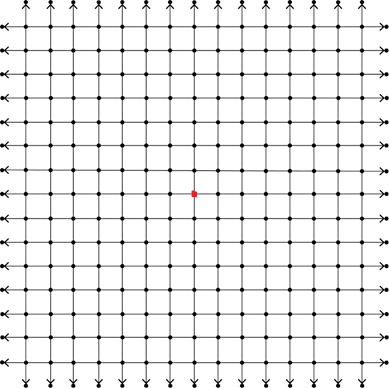
\includegraphics[scale=0.27]{game_field}
    }
    \caption{
        Рисунок 2. Решетка игрового поля, состоящая из внутренних узлов (серые) и граничных узлов (красные), по достижении которых происходит завершение игры.
    }\label{fig:game_field}
\end{figure}


\subsection{Поглощающие Марковские цепи}\label{subsec:ch1/sec3/sub2}

Расширенная теория поглощающих Марковских цепей является расширение стандартной теории и предоставляет возможности 
для расчета статистики времен поглощения \cite{kemeny1983}. 
Расширенная теория раскладывает матрицу переходов ${\rm P}$ в виде блочной матрицы:
\begin{equation}
    \begin{aligned}
    {\rm P}=
      \begin{bmatrix}
        Q & R \\
        {\bf 0} & I_r
      \end{bmatrix}
    \label{eq:P}
    \end{aligned}
\end{equation}
где $Q$ это матрица размера $s \times s$, характеризующая переходы между внутренними состояниями, 
$R$ -- ненулевая матрица размера $s \times r$, соответствующая переходам из внутренних состояний в поглощающие, 
$I_r$ -- единичная матрица размера $r \times r$, описывающая свойство петель в поглощающих состояниях, совместно с нулевой матрицей
${\bf 0}$ размера $r \times s$, указывающей на невозможность выхода из поглощающего состояния (поглощение) \cite{kemeny1983}.

Применяя многократно матрицу переходов для внутренних состояний и проводя суммирование результирующей матрицы по всем моментам времени,
теория поглощающих Марковских цепей вводит понятие фундаментальной матрицы $N$. Так как матрица $Q$ имеет норму меньшую единицы и является сжимающим отображением,
то соответствующий ряд сходится и имеет место следующая замкнутая форма вычисления фундаментальной матрицы:
\begin{equation}
    \begin{aligned}
    N=\sum_{k=0}^{\infty} Q^k=(I_s-Q)^{-1}
    \label{eq:N}
    \end{aligned}
\end{equation}
где $I_s$ это единичная матрица размера $s \times s$. Элемент фундаментальной матрицы $N$ с индексами $(i, j)$ 
является математическим ожиданием количества раз обнаружить цепь в состоянии $j$, при условии начала блуждания в состоянии $i$.

Используя свойство фундаментальной матрицы теория дает способ вычислить ожидаемое число шагов до поглощения
при условии начала блуждания в некотором внутреннем состоянии $i$:
\begin{equation}
    \begin{aligned}
    T=N{\bf 1}
    \label{eq:T}
    \end{aligned}
\end{equation}
где ${\bf 1}$ вектор все элементы которого единицы.

В рассматриваемой игровой механике стартовая позиция игры находится в центре решетки. 
Тогда соответствующее математическое ожидание числа ходов до поглощения ${\rm \bf t_n}$ ($n$ - размер поля) 
будет записано в элементе вектора $T$, соответствующем состоянию цепи с положением $(0, 0)$ на игровой решетке.

\subsection{Игра в терминах цепи Маркова}\label{subsec:ch1/sec3/sub3}

Игровая механика Random Walk Game предполагает игру двух оппонентов, на каждом ходу определяющих свой выбор одного из двух доступных вариантов.
В общем случае, каждый из игроков обладает памятью и может ориентироваться на предысторию ходов оппонента.
Формулировка игры в виде Марковского процесса позволяет одному из игроков вычислить равновесие Нэша в смешанных стратегиях \cite{}.
Наличие такого равновесия и независимость стратегии от номера хода одного игрока не позволит другому игроку использовать предысторию ходов
для получения большего выигрыша в среднем. Таким образом при оптимальной игре обоих игроков процесс будет являться Марковским.

Рассмотрим подробнее математическую формулировку в терминах поглощающих Марковских цепей игры Random Walk Game.
Независимая от номера хода стратегия игрока $S_{ij}^p$ описывается распределением Бернулли $\sigma_{ij}^p$ для игрока 
$p \in \{A, B\}$ в состоянии с координатами $(i, j)$:

\begin{equation}
    \begin{aligned}
    {\bf \sigma}_{ij}^p(s)=
    \begin{cases}
        f_{ij}^p, &\mbox{if } s = 0,\\ 
        1-f_{ij}^p, &\mbox{if } s = 1,\\
    \end{cases}
    \label{eq:sigma}
    \end{aligned}
\end{equation}

где $0 <= f_{ij}^p <= 1$ -- вероятность выбора игроком первого варианта хода $(s=0)$.

Определение движения фишки на поле осуществляется после выбора обоими игроками своего варианта хода в соответствии с правилами,
описанными в разделе \cref{Описание игры}. Движение возможно в одном из 4 направлений в соседние состояния:
$(i, j + 1), (i + 1, j), (i, j - 1), (i - 1, j)$. Результирующее направление определяется совместным распределением, 
задающим вероятность перехода из состояния $(i, j)$ в состояние $(x, y)$:
\begin{equation}
    \begin{aligned}
    P& \left( (i, j) \rightarrow (x, y) \right) = \\
    &=\begin{cases}
        0, &\mbox{if } |i-x|+|j-y| \neq 1,\\ 
        f_{ij}^A \left(1-f_{ij}^B\right), &\mbox{if } x=i \land y=j+1, {\bf \rightarrow}\\
        \left(1-f_{ij}^A\right) f_{ij}^B, &\mbox{if } x=i+1 \land y=j, {\bf \downarrow}\\
        \left(1-f_{ij}^A\right) \left(1-f_{ij}^B\right), &\mbox{if } x=i \land y=j-1, {\bf \leftarrow}\\
        f_{ij}^A f_{ij}^B, &\mbox{if } x=i-1 \land y=j, {\bf \uparrow}\\
    \end{cases}
    \label{eq:transition}
    \end{aligned}
\end{equation}

Первый случай в формуле определяет нулевую вероятность перехода между несвязанными состояниями, и оставшиеся соответствуют четырем направлениям движения фишки.

Два набора значений $f_{ij}^p, p \in \{A, B\}$ задает стратегию обоих игроков в каждом узле квадратной решетки $(i, j)$. 
Фиксация этих значений до начала игры позволяет вычислить матрицу вероятностей переходов между состояниями, то есть полностью определить Марковскую цепь.
Наиболее общий случай игры PvP позволяет обоим игрокам задавать свой набор вероятностей $f_{ij}^p$. В случае игры против среды PvE
стратегия одного из игроков известна и представляет собой равновероятный выбор среди двух возможных вариантов независимо от позиции на поле и номера хода:
$f_{ij}^{p_1} = 0.5, p_1 \in \{A, B\}$, а для второго игрока значения определяются произвольно $f_{ij}^{p_2}, p_2 \in \{A, B\} \setminus \{p_1\}$. 
Вырожденный случай игры BvB случайного блуждания определяется равновероятным выбором обоих игроков одного из вариантов хода $f_{ij}^{A} = f_{ij}^{B} = 0.5$
для всех состояний игры. В этом случае вероятность перехода из каждого внутреннего состояния в соседнее равно $1/4$.

Оба игрока рассматривают в качестве цели количество ходов в игре. Цель одного минимизировать количество ходов, а цель второго -- максимизировать.
В случае Марковской цепи при определенных смешанных стратегиях игроков целевой функцией является математическое ожидание времени достижения границы.
Обозначим соответствующие средние времена поглощения в игре для трех случаев как ${\bf t_n^{BvB}}$, ${\bf t_n^{PvE}}$ и ${\bf t_n^{PvP}}$.

\subsection{Моделирование эволюции вероятности}\label{subsec:ch1/sec3/sub3}

Аналитический подход теории поглощающих Марковских цепей позволяет вычислить значение среднего времени поглощения случайного блуждания
с применением матричных преобразований. Однако теории для расчета точного распределения времени поглощения в случае Марковских цепей
разработано не было. Прямой подход к расчету оценки распределения времени поглощения возможен благодаря математическому моделированию процесса 
эволюции вероятности. Дополнительным преимуществом данного подхода является возможность оценки наряду с распределением времени достижения также 
пространственного распределения вероятностей. 

Рассмотрим подробнее модель эволюции вероятности. Пусть $W_{ij}^{k}$ -- вероятность найти фишку в состоянии $(i, j)$ в момент времени $k$.
Начальное состояние игры в центре поля $(0, 0)$ соответствует единичной вероятности найти частицу в начальный момент времени $t=0$ в состоянии $(0, 0)$,
то есть $W_{0,0}^{0}=1$ и $W_{ij}^{0}=0$ для остальных состояний $((i, j) \neq (0, 0))$. Упорядочим все состояния последовательно по формуле $in + j$, где $n$ -- размер поля.
Тогда вектор ${\bf w^{0}}$ описывает распределение вероятности в начальный момент времени, а для всех моментов времени $k > 0$ 
распределения последовательно определяются по формуле эволюции вероятности:

\begin{equation}
    \begin{aligned}
    {\bf w^{k+1}}={\rm \widetilde{P}}{\bf w^{k}}, k \geq 0
    \label{eq:evolution}
    \end{aligned}
\end{equation}

где ${\rm \widetilde{P}}$ -- модифицированная матрица вероятностей переходов между состояниями цепи. 
Пропогация вектора вероятности на каждом шаге также дает возможность оценить точную вероятность $W_{ij}^{k}, (i, j) \in {\bf B}$ окончания блуждания на $k$-ом ходу
в граничном состоянии $(i, j)$. Для этого используется модифицированная матрица переходов такая, что при достижении границы фишкой 
происходит ее исключение из системы. Тогда вероятность поглощения частицы на $k$-ом шаге может быть вычислена по следующей формуле:

\begin{equation}
    \begin{aligned}
    p_{\rm abs}^{k}=\sum_{(i, j) \in {\bf B}} W_{ij}^{k},
    \label{eq:timedistr}
    \end{aligned}
\end{equation}
где ${\bf B}$ -- множество граничных состояний.

Моделирование эволюции вероятности также позволяет вычислить пространственное распределение вдоль граничных состояний за
счет аппроксимации ряда вероятностей поглощения в узле $(i, j) \in {\bf B}$ по всем моментам времени.
\begin{equation}
    \begin{aligned}
    p_{ij}^{\rm abs}=\sum_{k=0}^{\infty} W_{ij}^{k}
    \label{eq:spacedistr}
    \end{aligned}
\end{equation}

В связи с экспоненциальным убыванием вероятности $W_{ij}^{k}$ с ростом номера $k$ суммирование выполняется до достижения заданной точности
модуля разности между соседними членами.

Дополнительным свойством, представляющем интерес при анализе игровой динамики, является соотношение вероятностей
закончить игру на четном числе ходов или на нечетном. Отличие этого соотношения от единицы обусловлено 
тем, что четырехсвязная квадратная решетка представляет собой двудольный граф,
в связи с чем на каждом ходу фишка может находится только в одной из долей в зависимости от четности хода.
Обозначим долю графа четной, если фишка находится в ней на четном ходу, и нечетной -- если на нечетном ходу.
Состояния $(i, j)$ двух долей расположены на решетке в шахматном порядке и аналогично могут быть отнесены
к "четным" и "нечетным" состояниям в соответствии с четностью суммы координат $(i + j) \mod 2$.
Распространение вероятности по цепи происходит за счет полного перехода между долями. 
Однако вероятность поглощения в четных и нечетных состояниях отличается ввиду разного количества и расположения поглощающих состояний в долях.

Применение подхода к моделированию эволюции вероятности позволяет численно получить большой спектр информации о свойствах игры.

\subsection{Численное моделирование}\label{subsec:ch1/sec3/sub4}

Анализ статистических свойств игровой динамики возможен благодаря подходам, использующим теорию Марковских цепей
и моделирование эволюции вероятности. Однако исследование структурных особенностей индивидуальных траекторий 
требует применения методов численного моделирования. Одним из способов решения задачи является метод Монте-Карло
для симуляции случайного процесса с использованием генератора случайных чисел. Сталкивая различные смешанные стратегии,
исследуемые в ходе работы, возможно построить последовательность перемещений фишки по решетке, движущейся в соответствии
с правилами игры. Алгоритм симуляции состоит из нескольких шагов:

\item Начальное положение фишки определяется в центре поля $(0, 0)$. 
\item На каждом ходе генерируются выборы игроков из распределения с соответствующей стратегией игрока
с использованием псевдослучайного генератора Mersenne Twister из модуля random в Python 3.8.
\item В соответствие с правилами перехода фишка перемещается в одно из соседних состояний.
\item По достижении фишкой одного из граничных состояний симуляция останавливается.

В результате работы алгоритма генерируется последовательность ходов игроков и движений фишки на поле.
Для визуализации индивидуальных траекторий реализованы три способа: 
\item визуализация всех ходов траектории с наложением на одной плоскости
\item разбиение ходов на последовательные группы по 40 ходов и визуализация групп блоками от первой до очередной группы.
\item анимация движения фишки и след траектории с затуханием.

Дополнительно, при сравнении с результатами моделирования эволюции вероятности были вычислены частоты
встречаемости времен полученных игр. 

\subsection{Полевой эксперимент}\label{subsec:ch1/sec3/sub6}

Математический подход к анализу стратегий дает возможность выявить наиболее оптимальные 
способы действия игроков. Однако в реальных условиях на поведение человека, принимающего решение
о конкретном ходе, влияет большой спектр факторов: настроение, предыдущие действия игроков, внешние обстоятельства и т.д.
Естественный подход к продолжению анализа игровой динамики состоит в проведении полевого эксперимента
с участием людей в качестве игроков. 

Для участия в эксперименте были приглашены волонтеры в возрасте от 16 до 52 лет. 
Игроки до 25 лет были отобраны из числа студентов ННГУ им. Н.И.Лобачевского и Высшей школы экономики. 
Игроки старше 25 лет были набраны из разных университетов и исследовательских институтов России, Германии, Норвегии и Южной Кореи.

Основной критерий для отбора участников состоял в основном роде деятельности заключающемся в умственном труде.
Большая часть участников представляет собой успешных студентов, призеров олимпиад, профессоров, кандидатов наук, успешных ИТ-специалистов.

Проведение эксперимента состояло из четырех отдельных мероприятий:
\item Организованные игры без конкурса между участниками.
    Студенты находились в одной комнате и играли не общаясь друг с другом в течение одного часа. 
    Интерес участников заключался в достижении самой длинной игры среди участников. 
    Пары игроков выбирались на основе схожести их навыков в олимпиадном программировании.
\item Конкурс на получение наибольшего количества очков при игре против среды PvE.
    Участники играли онлайн в течение месяца соревнуясь с другими участниками в общем рейтинге.
    Рейтинг представлял собой отношение двух экспоненциально скользящих средних длительностей по играм за центр и за границу.
    Общий рейтинг все время был доступен участникам.
\item Личный чемпионат между студентами в играх PvP: 
    Студенты находились в одной аудитории и играли не общаясь друг с другом в течение двух часов. 
    Участники распределялись по взвешенной сумме длин сыгранных игр. 
    Чем длиннее игра - тем выше вес, связанный с этой игрой для участника, играющего за центр (A) и противоположный для участника, играющего за границу (B).
    Интерес участников заключался в получении наивысшего места в таблице.
\item Свободные игры без конкурса между участниками и между участником и средой.
      Участники находились дома и играли не общаясь около 30 минут в день. 
      Интерес участников состоял в получении наибольшего (наименьшего) счета в конкретной игре.
      В любой момент игроки могли приостановить игру и продолжить ее в удобное для них время.

Цели игроков распределялись между ними равновероятно на основе генератора случайных чисел.

\subsection{Мобильное приложение и архитектура системы}\label{subsec:ch1/sec3/sub6}

Для организации экспериментальной части было разработано мобильное приложение, 
доступное в Google Play Store (https://play.google.com/store/apps/details?id=com.scigames.RWGame) и 
в AppStore (https://apps.apple.com/us/app/random-walk/id1564589250). Приложение предоставляет два режима игры: 
игра против другого игрока (PvP) или игра против среды (PvE). В обоих режимах приложение отправляет выбор игроков 
через Интернет на веб-сервер и рассчитывает направление и следующую позицию фишки на поле. Результаты игр 
(траектории и соответствующие выборы стратегий игроков на каждом ходу) были собраны в базе данных на сервере для дальнейшего анализа.

Выбор одной из двух стратегий среды в режиме PvE определяется последовательностью псевдослучайных чисел, 
вычисленных генератором случайных чисел Mersenne Twister (реализованным в PHP 7.4 как функция mt_rand) \cite{}. 
Игры, полученные в эксперименте, проводились на  поле размера 17×17.

Архитектура системы состоит из трех основных компонент: мобильное приложение, веб-сервер и база данных.
Взаимодействие между мобильным приложением и веб-сервером осуществляется посредством REST API по защищенному протоколу HTTPS
через сеть Интернет. Процесс взаимодействия клиента и сервера состоит из нескольких этапов:
\item Пользователь осуществляет регистрацию в системе, информация о регистрации отправляется на веб-сервер и сохраняется в БД.
\item Пользователь аутентифицируется в системе на основе связки логин и пароль, либо на основе OAuth аутентификации.
\item Успешная аутентификация авторизует пользователя в системе и предоставляет список текущих игр пользователя, историю игр пользователя, рейтинг участников, и возможность начать новую игру.
\item Игрок инициирует игру с другим игроком по логину, случайным образом или выбором незавершенной игры из списка.
\item После инициализации двумя игроками одной и той же игры, выбранная каждым игроком стратегия на ходе передается на веб-сервер и сохраняется в БД.
\item Клиент опрашивает веб-сервер до тех пор, пока оба игрока не совершат выбор в текущем ходе.
\item После совершения выбора обоими игроками веб-сервер определяет направление движения фишки, факт достижения границы и по запросу передает на клиент эту информацию.
\item На клиенте обновляется положение фишки, количество ходов. Игра переходит на следующий ход или завершается.

В качестве HTTP-сервера используется веб-сервер nginx \cite{}. Программная часть, реализующая функционал серверной части, 
разработана на языке PHP 7.4 \cite{} без использования дополнительных фреймворков с использованием модели Model-View-Controller (MVC) \cite{}. 
Хранение информации реализовано на основе реляционной базы данных MySQL с применением хранимых процедур для защиты от XSS атак к базе данных \cite{}.
Защита паролей осуществляется с применением хеширования с солью на основе алгоритма bcrypt (реализовано в PHP 7.4 как функция password_hash).

Мобильное приложение разработано с применением технологии Xamarin на языке C# \cite{}. Преимуществом данной технологии в сравнении с 
другими, такими как Kotlin в среде разработки Android Studio, Objective-C, Swift в среде разработки XCode, является кроссплатформенность
при сохранении общей кодовой базы бизнес-логики и возможности индивидуализации интерфейса пользователя по конкретную платформу.
Xamarin предлагает три платформы для сборки приложения: Universal Windows App, Android, iOS. Наличие широкого выбора компонент,
оптимизированных для разных платформ, позволило в короткие сроки разработать мобильное приложение для трех платформ.
Основным паттерном проектирования приложения был выбран подход Model-View-ViewModel (MVVM). Разделение приложения на логически
связанные компоненты и построение качественной архитектуры позволило сделать приложение гибким к внесению дополнительных изменений.

\section{Выводы по главе 2}\label{sec:ch2/sec4}

В данной главе были рассмотрены алгоритмы и методы исследования, примененные для анализа 
предложенной игры в терминах Марковских процессов. Получено описание игрового процесса 
с использованием аппарата поглощающих Марковских цепей и смешанных стратегий.
Предложенные методы реализованы с использованием языка Python 3.8 и библиотек numpy, scipy, matplotlib.
Разработано и реализовано мобильное приложение 